%preamble - package unclusion and set up
\documentclass[12pt,twoside,a4paper]{report}
\usepackage{etex}
% Select encoding of your inputs.
\usepackage[utf8]{inputenc}

% Make latex understand and use the typographic
% rules of the language used in the document.
\usepackage[english]{babel}

% Use the vector font Latin Modern which is going
% to be the default font in latex in the future.
\usepackage{lmodern}

% Choose the font encoding
\usepackage[T1]{fontenc}

% Use colour in tables
\usepackage[table]{xcolor}
\usepackage{array}
\usepackage{multirow}

% load a colour package
\usepackage{xcolor}
\definecolor{aaublue}{RGB}{33,26,82}% dark blue

% The standard graphics inclusion package
\definecolor{white}{RGB}{255,255,255} % define color white
\usepackage{graphicx}
\usepackage{adjustbox}

% Set up how figure and table captions are displayed
\usepackage{caption}
\captionsetup{
  font=footnotesize,% set font size to footnotesize
  labelfont=bf % bold label (e.g., Figure 3.2) font
}

% Enable row combination in tables
\usepackage{multirow}

% Make space between table lines and text
\renewcommand{\arraystretch}{1.5}

% Enable commands like \st (strike out) and \hl (high light)
\usepackage{soul}

% Make the standard latex tables look so much better
\usepackage{array,booktabs}

% Enable the use of frames around, e.g., theorems
% The framed package is used in the example environment
\usepackage{framed}
\usepackage{colortbl}
\usepackage{longtable}
\usepackage{xcolor}
\usepackage{textcomp}

%%%%%%%%%%%%%%%%%%%%%%%%%%%%%%%%%%%%%%%%%%%%%%%%
% Mathematics
%%%%%%%%%%%%%%%%%%%%%%%%%%%%%%%%%%%%%%%%%%%%%%%%
% Defines new environments such as equation,
% align and split 
\usepackage{amsmath}
\usepackage{relsize}
% Adds new math symbols
\usepackage{amssymb}
% Use theorems in your document
% The ntheorem package is also used for the example environment
% When using thmmarks, amsmath must be an option as well. Otherwise \eqref doesn't work anymore.
\usepackage[framed,amsmath,thmmarks]{ntheorem}

%%%%%%%%%%%%%%%%%%%%%%%%%%%%%%%%%%%%%%%%%%%%%%%%
% Page Layout
%%%%%%%%%%%%%%%%%%%%%%%%%%%%%%%%%%%%%%%%%%%%%%%%
% Change margins, papersize, etc of the document
\usepackage[
  left=25mm,% left margin on an odd page %tidligere 25mm for baade right og left
  right=25mm,% right margin on an odd page
  top=35mm,
  ]{geometry}
  
% Modify how \chapter, \section, etc. look
% The titlesec package is very configureable
\usepackage{titlesec}
\makeatletter
\def\ttl@mkchap@i#1#2#3#4#5#6#7{%
    \ttl@assign\@tempskipa#3\relax\beforetitleunit
    \vspace{\@tempskipa}%<<<<<< REMOVE THE * AFTER \vspace
    \global\@afterindenttrue
    \ifcase#5 \global\@afterindentfalse\fi
    \ttl@assign\@tempskipb#4\relax\aftertitleunit
    \ttl@topmode{\@tempskipb}{%
        \ttl@select{#6}{#1}{#2}{#7}}%
    \ttl@finmarks  % Outside the box!
    \@ifundefined{ttlp@#6}{}{\ttlp@write{#6}}}
\makeatother

\titlespacing{\chapter}{0pt}{0pt}{10pt}
\titlespacing{\section}{0pt}{0pt}{-5pt}
\titlespacing{\subsection}{0pt}{8pt}{-5pt}
\titlespacing{\subsubsection}{0pt}{6pt}{-10pt}

\titleformat*{\section}{\normalfont\Large\bfseries\color{aaublue}}
\titleformat*{\subsection}{\normalfont\large\bfseries\color{aaublue}}
\titleformat*{\subsubsection}{\normalfont\normalsize\bfseries\color{aaublue}}

\usepackage{titlesec, blindtext, color}
%\color{gray75}{gray}{0.75}
\newcommand{\hsp}{\hspace{20pt}}
\titleformat{\chapter}[hang]{\Huge\bfseries}{\thechapter\hsp\textcolor{aaublue}{|}\hsp}{0pt}{\Huge\bfseries}

% Change the headers and footers
\usepackage{fancyhdr}
\setlength{\headheight}{15pt}
\pagestyle{fancy}
\fancyhf{} %delete everything
\renewcommand{\headrulewidth}{0pt} %remove the horizontal line in the header
\fancyhead[RO,LE]{\color{aaublue}\small\nouppercase\leftmark} %even page - chapter title
\fancyhead[LO]{}
\fancyhead[RE]{} 
\fancyhead[CE]{}
\fancyhead[CO]{}
\fancyfoot[RE,LO]{\thepage}
\fancyfoot[LE,RO]{Gr. 834} %page number on all pages
\fancyfoot[CE,CO]{}

% change first page of all chapters header and footer to fancy style
\makeatletter
\let\ps@plain\ps@fancy
\makeatother

% Do not stretch the content of a page. Instead,
% insert white space at the bottom of the page
\raggedbottom

% Enable arithmetics with length. Useful when typesetting the layout.
\usepackage{calc}

%%%%%%%%%%%%%%%%%%%%%%%%%%%%%%%%%%%%%%%%%%%%%%%%
% Bibliography
%%%%%%%%%%%%%%%%%%%%%%%%%%%%%%%%%%%%%%%%%%%%%%%%
%setting references (using numbers) and supporting i.a. Chicargo-style:
%\usepackage[citestyle=authoryear,natbib=true]{biblatex}
\usepackage[backend=biber]{biblatex}
%\usepackage{etex}
%\usepackage{etoolbox}
%\usepackage{keyval}
%\usepackage{ifthen}
%\usepackage{url}
%\usepackage{csquotes}
%\usepackage[backend=biber, url=true, doi=true, style=numeric, sorting=none]{biblatex}
%\addbibresource{setup/bibliography.bib}
\bibliography{setup/bibliography.bib}

\usepackage[utf8]{inputenc}
\usepackage[english]{babel}

\usepackage{comment}

%\usepackage[
%backend=biber,
%style=numeric,
%sorting=ynt
%]{biblatex}
%\addbibresource{setup/bibliography.bib}

%%%%%%%%%%%%%%%%%%%%%%%%%%%%%%%%%%%%%%%%%%%%%%%%
% Misc
%%%%%%%%%%%%%%%%%%%%%%%%%%%%%%%%%%%%%%%%%%%%%%%%

%%% Enables the use FiXme refferences. Syntax: \fxnote{...} %%%
\usepackage[footnote, draft, english, silent, nomargin]{fixme}
%With "final" instead of "draft" an error will ocure for every FiXme under compilation.

%%% allows use of lorem ipsum (generate i.e. pagagraph 1 to 5 with \lipsum[1-5]) %%%
\usepackage{lipsum}

%%% Enables figures with text wrapped tightly around it %%%
\usepackage{wrapfig}

%%% Section debth included in table of contents (1 = down to sections) %%%
\setcounter{tocdepth}{1}

%%% Section debth for numbers (1 = down to sections) %%%
\setcounter{secnumdepth}{1}

\usepackage{tocloft}
\setlength{\cftbeforetoctitleskip}{0 cm}
\renewcommand{\cftpartpresnum}{Part~}
\let\cftoldpartfont\cftpartfont
\renewcommand{\cftpartfont}{\cftoldpartfont\cftpartpresnum}

%%%%%%%%%%%%%%%%%%%%%%%%%%%%%%%%%%%%%%%%%%%%%%%%
% Hyperlinks
%%%%%%%%%%%%%%%%%%%%%%%%%%%%%%%%%%%%%%%%%%%%%%%%

% Enable hyperlinks and insert info into the pdf
% file. Hypperref should be loaded as one of the 
% last packages
\usepackage{nameref}
\usepackage{hyperref}
\hypersetup{%
	%pdfpagelabels=true,%
	plainpages=false,
	pdfauthor={Author(s)},%
	pdftitle={Title},%
	pdfsubject={Subject},%
	bookmarksnumbered=true,%
	colorlinks,%
	citecolor=aaublue,%
	filecolor=aaublue,%
	linkcolor=aaublue,% you should probably change this to black before printing
	urlcolor=aaublue,%
	pdfstartview=FitH%
}

% remove all indentations
\setlength\parindent{0pt}
\parskip 5mm
\usepackage{verbatim}

\definecolor{Gra}{RGB}{230,230,230}

%creates a nice-looking C#-text
\newcommand{\CC}{C\nolinebreak\hspace{-.05em}\raisebox{.3ex}{\scriptsize\text \#} }

%enables multi column lists
\usepackage{multicol}

%enables code-examples
\usepackage{listings}

\definecolor{coolblue}{RGB}{32,95,128}
\definecolor{mygreen}{rgb}{0,0.6,0}
\definecolor{mygray}{rgb}{0.5,0.5,0.5}
\definecolor{mymauve}{rgb}{0.58,0,0.82}
\usepackage{textcomp}
\definecolor{listinggray}{gray}{0.9}
\definecolor{lbcolor}{rgb}{0.9,0.9,0.9}

\lstset{
backgroundcolor=\color{lbcolor},
	tabsize=4,
	rulecolor=,
	language=C,
        basicstyle=\scriptsize,
        upquote=true,
        aboveskip={1.5\baselineskip},
        columns=fixed,
        showstringspaces=false,
        extendedchars=true,
        breaklines=true,
        prebreak = \raisebox{0ex}[0ex][0ex]{\ensuremath{\hookleftarrow}},
        frame=single,
        showtabs=false,
        numbers=left,
        captionpos=b,
        numbersep=5pt,
        numberstyle=\tiny\color{mygray},
        showspaces=false,
        showstringspaces=false,
        identifierstyle=\ttfamily,
        keywordstyle=\color[rgb]{0,0,1},
        commentstyle=\color[rgb]{0.133,0.545,0.133},
        stringstyle=\color[rgb]{0.627,0.126,0.941},
}

%% ADD MATLAB COLOR CODE
\lstdefinestyle{custommatlab}{
	backgroundcolor=\color{lbcolor},
	tabsize=4,
	rulecolor=,
	language=Matlab,
	basicstyle=\scriptsize,
	upquote=true,
	aboveskip={1.5\baselineskip},
	columns=fixed,
	showstringspaces=false,
	extendedchars=true,
	breaklines=true,
	prebreak = \raisebox{0ex}[0ex][0ex]{\ensuremath{\hookleftarrow}},
	frame=single,
	showtabs=false,
	numbers=left,
	captionpos=b,
	numbersep=5pt,
	numberstyle=\tiny\color{mygray},
	showspaces=false,
	showstringspaces=false,
	identifierstyle=\ttfamily,
	keywordstyle=\color[rgb]{0,0,1},
	commentstyle=\color[rgb]{0.133,0.545,0.133},
	stringstyle=\color[rgb]{0.627,0.126,0.941},   
}
\lstdefinestyle{custommatlabinline}{
	style=custommatlab,
	basicstyle=\small,
}

\usepackage{float}
\usepackage{caption}
\usepackage{subcaption}
\usepackage{siunitx}
\sisetup{decimalsymbol=comma}
\sisetup{detect-weight}

\usepackage{enumitem}

% Figures - TIKZ
\usepackage{tikz}
\usetikzlibrary{shapes,arrows}
\usepackage[americanresistors,americaninductors,americancurrents, americanvoltages]{circuitikz}

% Wall of text logo
\newcommand{\walloftextalert}[0]{\includegraphics[width=\textwidth]{walloftext.png}}

\usepackage{pdfpages}
\usepackage{lastpage}
\usepackage{epstopdf}

\setlength{\headheight}{21pt}

\hfuzz=\maxdimen
\tolerance = 10000
\hbadness  = 10000

\usepackage{siunitx}
\graphicspath{{./figures/}}

\usepackage{todonotes}

\usepackage{nomencl}
\makenomenclature


\usepackage[toc,xindy]{glossaries}
\makeglossaries


\usepackage{ifthen}
\renewcommand{\nomgroup}[1]{%
	\ifthenelse{\equal{#1}{T}}{\item[\textbf{\Large Terminology}]}{%
	\ifthenelse{\equal{#1}{A}}{\item[\textbf{\Large Acronyms}]}{%
	\ifthenelse{\equal{#1}{R}}{\item[\textbf{\Large Reference Frames}]}{%
	\ifthenelse{\equal{#1}{S}}{\item[\textbf{\Large Symbols}]}{}}
}}}

\setlength{\nomlabelwidth}{4.5cm} % set spacing between symbol and description

\renewcommand{\nompreamble}{
	\section*{Notations}

Vectors used have a bold typeface.  
\begin{equation*}
\textbf{v}
\end{equation*}
Matrices are underlined.
\begin{equation*}
\underline{A}
\end{equation*}

Cross product operations can be evaluated by taking the skew symmetric matrix of the left vector and executing a matrix multiplication. The skew symmetric matrix of $\textbf{v}$ is denoted as $\underline{v}^\times$
\begin{equation*}
	\textbf{w} = \textbf{u} \times \textbf{v} = \underline{u}^\times \textbf{v}
\end{equation*}
Matrix transposition is denoted as
\begin{equation*}
\underline{A}^T
\end{equation*}
If a non-square matrix has to undergo an operation similar to inversion, Moore-Penrose pseudoinverse is used. Pseudoinverse matrix is indicated as $\underline{A}^\dagger$. If the matrix satisfies $rank(\underline{A}) = min(m,n)$ and $m < n$, the left pseudoinverse is used as follows
\begin{equation*}
\underline{A}^\dagger    =   (\underline{A}^T \underline{A} )^{-1} \underline{A}^T 
\end{equation*}

If $n < m$, the right pseudoinverse is used as follows

\begin{equation*}
 \underline{A}^\dagger    =  \underline{A}^T  (\underline{A} \underline{A}^T)^{-1}
\end{equation*}


The majority of equations are expressed in body-fixed frame (BFF). Unless it's not explicitly noted, the matrices and vectors are expressed in BFF. In case the expression is in earth centered inertial frame (ECI), it is noted in the superscript as 

\begin{equation*}
\vec{XY}^{[I]}
\end{equation*}

The rotation quaternion between frames use the subscript to denote the frame where the transformation is done from, the superscript is the symbol of the frame being transformed into. In case the frame symbols are not present, it should be interpreted as a transformation from inertial frame to body frame.

\begin{equation*}
\vec{^s_i q(t)}
\end{equation*}

Rotation matrix corresponding to rotation matrix $\vec{^s_i q(t)}$ is denoted as
\begin{equation*}
\underline{R}(\vec{^s_i q(t)})
\end{equation*}}

%macros - please read this file
%%%%%%%%%%%%%%%%%%%%%%%%%%%%%%%%%%%%%%%%%%%%%%%%%%%%%
%             UNITS, EQUATIONS AND TEXT             %
%%%%%%%%%%%%%%%%%%%%%%%%%%%%%%%%%%%%%%%%%%%%%%%%%%%%%
%Units:
\newcommand{\unit}[1]{&& \left[\si{#1}\right]} %\newcommand{\unit}[1]{[\si{#1}]}             <<| Use these if you want equations to be
\newcommand{\unitWh}[1]{[\si{#1}]}             %\newcommand{\eq}[2]{&&\si{#1} &= \si{#2}&&}  <<| centered.. .. will appear scrambled
\newcommand{\numUnit}[1]{\ \si{#1}&}           %                                               | from one equation to the next though..
%Equation:                                     %                                               | and does not work with long equations.. :/
\newcommand{\eq}[2]{\si{#1} &= \si{#2}}
\newcommand{\arw}{&& &\Updownarrow&&}
\newcommand{\eqOne}[2]{\si{#1} &= \si{#2} &\nonumber\\}
\newcommand{\eqTwo}[1]{&\ \ \ \ \si{#1}&}
%Text:
\newcommand{\tx}[1]{\text{#1}}
%Vectors
\renewcommand{\vec}[1]{\boldsymbol{\mathbf{#1}}}
%Vertical line in equations ie. |_x=y (whereTwo stacks two equalities at the line)
\newcommand{\where}[1]{ \left.\rule{0cm}{.5cm}\right\vert\rule{0cm}{.4cm}_{\substack{\rule{0cm}{.15cm}\\ \si{#1} }} }
\newcommand{\whereTwo}[2]{ \left.\rule{0cm}{.67cm}\right\vert\rule{0cm}{.5cm}_{\substack{\si{#1} \rule{0cm}{.19cm}\\\vspace{-.1cm}\\ \si{#2}}} }

%%%%%%%%%%%%%%%%%%%%%%%%%%%%%%%%%%%%%%%%%%%%%%%%%%%%%
%                 TIKZ SETTINGS                     %
%%%%%%%%%%%%%%%%%%%%%%%%%%%%%%%%%%%%%%%%%%%%%%%%%%%%%
\tikzset{
  block/.style    = {draw, thick, rectangle,
                     minimum height = 3em,
                     minimum width = 3em},
  sum/.style      = {draw, circle}, % Adder
}

%%%%%%%%%%%%%%%%%%%%%%%%%%%%%%%%%%%%%%%%%%%%%%%%%%%%%
%                  REFERENCES                       %
%%%%%%%%%%%%%%%%%%%%%%%%%%%%%%%%%%%%%%%%%%%%%%%%%%%%%

%Chapter
\newcommand{\Chapref}[1]{\emph{Chapter \ref{#1}}}
\newcommand{\chapref}[1]{\emph{chapter \ref{#1}}}
%Section
\newcommand{\Secref}[1]{\emph{Section \ref{#1}}}
\newcommand{\secref}[1]{\emph{section \ref{#1}}}
%subSection
\newcommand{\Subsecref}[1]{\emph{Subsection \ref{#1}}}
\newcommand{\subsecref}[1]{\emph{subsection \ref{#1}}}
%Appendix
\newcommand{\Appref}[1]{\emph{Appendix \ref{#1}}}
\newcommand{\appref}[1]{\emph{appendix \ref{#1}}}
%Listings
\newcommand{\Coderef}[1]{\emph{Listings: \ref{#1}}}
\newcommand{\coderef}[1]{\emph{listings: \ref{#1}}}
%Figure:
\newcommand{\Figref}[1]{\emph{Figure \ref{#1}}}
\newcommand{\figref}[1]{\emph{figure \ref{#1}}}
%Table:
\newcommand{\Tableref}[1]{\emph{Table \ref{#1}}}
\newcommand{\tableref}[1]{\emph{table \ref{#1}}}

%Expressions:
\newcommand{\Expr}[1]{\emph{Expression (\ref{#1})}}
\newcommand{\expr}[1]{\emph{expression (\ref{#1})}}

%Equations:
%1 equation:
\newcommand{\Eqref}[1]{\emph{Equation (\ref{#1})}}
\renewcommand{\eqref}[1]{\emph{equation (\ref{#1})}}
%2 equations:
\newcommand{\EqrefTwo}[2]{\emph{Equation (\ref{#1})} and \emph{(\ref{#2})}}
\newcommand{\eqrefTwo}[2]{\emph{equation (\ref{#1})} and \emph{(\ref{#2})}}
%3 equations:
\newcommand{\EqrefThree}[3]{\emph{Equation (\ref{#1})}, \emph{(\ref{#2})} and \emph{(\ref{#3})}}
\newcommand{\eqrefThree}[3]{\emph{equation (\ref{#1})}, \emph{(\ref{#2})} and \emph{(\ref{#3})}}
%4 equations:
\newcommand{\EqrefFour}[4]{\emph{Equation (\ref{#1})}, \emph{(\ref{#2})}, \emph{(\ref{#3})} and \emph{(\ref{#4})}}
\newcommand{\eqrefFour}[4]{\emph{equation (\ref{#1})}, \emph{(\ref{#2})}, \emph{(\ref{#3})} and \emph{(\ref{#4})}}
%5 equations:
\newcommand{\EqrefFive}[5]{\emph{Equation (\ref{#1})}, \emph{(\ref{#2})}, \emph{(\ref{#3})}, \emph{(\ref{#4})} and \emph{(\ref{#5})}}
\newcommand{\eqrefFive}[5]{\emph{equation (\ref{#1})}, \emph{(\ref{#2})}, \emph{(\ref{#3})}, \emph{(\ref{#4})} and \emph{(\ref{#5})}}
%6 equations:
\newcommand{\EqrefSix}[6]{\emph{Equation (\ref{#1})}, \emph{(\ref{#2})}, \emph{(\ref{#3})}, \emph{(\ref{#4})}, \emph{(\ref{#5})} and \emph{(\ref{#6})}}
\newcommand{\eqrefSix}[6]{\emph{equation (\ref{#1})}, \emph{(\ref{#2})}, \emph{(\ref{#3})}, \emph{(\ref{#4})}, \emph{(\ref{#5})} and \emph{(\ref{#6})}}
%7 equations:
\newcommand{\EqrefSeven}[7]{\emph{Equation (\ref{#1})}, \emph{(\ref{#2})}, \emph{(\ref{#3})}, \emph{(\ref{#4})}, \emph{(\ref{#5})}, \emph{(\ref{#6})} and \emph{(\ref{#7})}}
\newcommand{\eqrefSeven}[7]{\emph{equation (\ref{#1})}, \emph{(\ref{#2})}, \emph{(\ref{#3})}, \emph{(\ref{#4})}, \emph{(\ref{#5})}, \emph{(\ref{#6})} and \emph{(\ref{#7})}} % :TIP: If you are using TeXstudio you can open
                         %     the file by Ctrl+LeftClick on setup/macros.tex
\begin{document}         %     If the file doesn't exist, you will be asked
angle constraint of the robot in robot describtion

Page 4, Robot Arm: A point P is mentioned.
Point P refers to the point in the end-effector that the robot will place where the object is.
\begin{figure}[H]
	\centering
	\includegraphics[width=0.8\linewidth]{figures2/arm}
	\caption{The measurements of the Crust Crawler. In the picture the Crust Crawler robot is seen in an upright position to show its full length. The point P shows the point that has to be aligned with the object for pickup.}
	\label{fig:arm}
\end{figure}


Page 8. section 4.1:
The third DH case is wrong it has to be:\\
- if $z_i$ and $z_{i-1}$ intersect, then $x_i$ is normal to the plane formed by if $z_i$ and $z_{i-1}$.
%\pagestyle{empty} %disable headers and footers
%\pagenumbering{roman} %use roman page numbering in the frontmatter I II...
%\fancyfoot[RE,LO]{17gr834} %page number on all pages
%\fancyfoot[LE,RO]{\thepage}
%\fancyhead[LE,LO,RE,RO]{}
%
%\pdfbookmark[0]{Front Page}{label:forside}%
\begin{titlepage}
  \addtolength{\hoffset}{0.5\evensidemargin-0.5\oddsidemargin} %set equal margins on the frontpage - remove this line if you want default margins
  \noindent%
  \begin{tabular}{@{}p{\textwidth}@{}}
    \toprule[2pt]
    \midrule
    \vspace{0.2cm}
    \begin{center}
    \Huge{\textbf{
      % CubeSat Formation Flying
      Fault Tolerant Attitude Control of a Pico-Satellite Equipped with Reaction Wheels
      and Magnetorquers% insert your title here
    }}
    \end{center}
%    \begin{center}
%      \Large{
%
%      }
%    \end{center}
    \vspace{0.2cm}\\
    \midrule
    \toprule[2pt]
  \end{tabular}
   \vspace{0.55 cm}
  \begin{figure}[!ht]
\centering
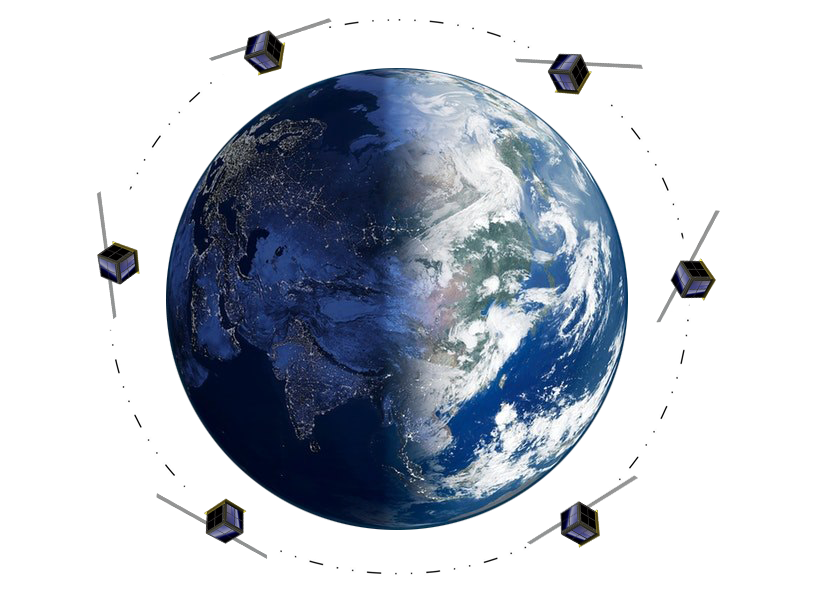
\includegraphics[width=0.8\textwidth]{figures/c1}
\label{fig:forside}
\end{figure}
  \vspace{0.6 cm}
  \begin{center}
%    {\large
%      2. Semester Project Report %Insert document type (e.g., Project Report)
%    }\\
    \vspace{0.2cm}
    {\Large
      Group 18gr1033 %Insert your group name or real names here
    }
  \end{center}
  \begin{center}
  Aalborg University\\
  Control \& Automation\\
  Fredrik Bajers Vej 7\\
  DK-9220 Aalborg
  \end{center}
\end{titlepage}

\clearpage	%frontpage doh
%\cleardoublepage
%%\begin{document} 
%\thispagestyle{empty}
%\begin{titlepage}
\begin{nopagebreak}
{\samepage 

\begin{tabular}{r}
\parbox{\textwidth}{  \raisebox{-15mm}{
\includegraphics[height=3cm]{figures/aaulogo-en.png}}
\hfill \hspace{2cm} \parbox{8cm}{\begin{tabular}{l} %4.90
{\small \textbf{\textcolor{aaublue}{\colorbox{white}{10\textsuperscript{th} Semester, Project}}}}\\
{\small \textbf{\textcolor{aaublue}{Technical Faculty of IT and Design}}}\\
{\small \textbf{\textcolor{aaublue}{Department of
	Electronics Systems}}}\\ 
{\small \textbf{\textcolor{aaublue}{Control and Automation}}}\\
{\small \textcolor{aaublue}{Fredrik Bajers Vej 7C}} \\
{\small \textcolor{aaublue}{9220 Aalborg}} \\
{\small \textcolor{aaublue}{\emph{en.aau.dk/education/master/control-automation}}}
\end{tabular}}}
\end{tabular}

\begin{tabular}{cc}
\parbox{7cm}{

\textbf{Title:}

Fault Tolerant Attitude Control of a Pico-Satellite Equipped with Reaction Wheels
and Magnetorquers \\ %\fxnote{Input project title}\\

\textbf{Theme:}

\small{
 Master thesis\\
}


\parbox{8cm}{


\textbf{Project Period:}\\
P10, Spring 2018\\
01/02/2018 - 07/06/2018\\
   
\textbf{Project Group:}\\
18gr1033\\ %\fxnote{Input group number}
  
\textbf{Participants:}\\
- Dániel Bolgár  \\
- Nikolaos Biniakos\\
- Alexandru-Cosmin Nicolae\\

\textbf{Supervisors:}\\
Jesper Abilgaard Larsen \\ %\fxnote{Input supervisor}
}\\


\textbf{Pages:} \\
\textbf{Appendices:} 2 (4 pages)\\
\textbf{Attached:} 1 zip file\\
\textbf{Concluded:} 07/06/2018\\

\vfill } &
\parbox{7cm}{
  \vspace{.15cm}
  \hfill
  \begin{tabular}{l}
  {\textbf{Synopsis}}\bigskip \\
  \fbox{
    \parbox{6.5cm}{\bigskip
     {\vfill{\small This report describes the design and simulation of a control system on a AAU-CubeSat, which is a pico- satellite used for Low Earth Orbit flight.

The objective is to use a flight formation for monitoring Greenland, by having eight satellites equally distributed in orbit.

Two controllers must be designed, one to control the angle between the satellites using the drag force, and one for attitude control.  The drag force applied on the satellite depends on the cross section area which can be controlled using the orientation of the satellite.

A linear and a non-linear control method have been designed in order to compare the differences between them.  
     \bigskip}}
     }}
   \end{tabular}}
\end{tabular}} %\vspace{1cm}



\end{nopagebreak}
%\end{titlepage}
%\end{document}
%\cleardoublepage
%\chapter*{Preface}
This report has been written by group 1033 during fourth semester in Control and Automation MSc in Aalborg University, Department of Electronic Systems during the period from February 2018 to June 2018. It is written as a Master's thesis for the Control and Automation Master's program. 

A nomenclature is included presenting the acronyms, symbols and terminology used throughout the thesis.  Quotes are inside quotation marks and are cursive.

The authors would like to thank Associate Professor Jesper Abilgaard Larsen for supervising. The authors furthermore would like to thank the students involved in the development of the AAUSAT Simulink Library.

% References made before a full stop regards the sentence and reference after full stop regards the paragraph.
Attached to report is a zip file with:
\begin{itemize}
	\item The MATLAB code 
	\item Simulink models
\end{itemize}
\vspace{2cm}

\textbf{Report by:}\\
\vspace{-5pt}
\begin{table}[H]
	\centering
	\begin{tabular}{c c c}
		\underline{\phantom{JAERJAERJAERJAERGO}} & \phantom{cookies} & \underline{\phantom{JAERJAERJAERJAERGO}} \\
		 	Dániel Bolgár	& \phantom{cookies} &  Nikolaos Biniakos	\\
		&&\\
		\multicolumn{3}{c}{\underline{\phantom{JAERJAERJAERJAERGO}}}\\
		\multicolumn{3}{c}{Alexandru-Cosmin Nicolae}\\				
						
	\end{tabular}
\end{table}


\pagebreak

%
%\tableofcontents         %     weather or not you want to create it.
%\cleardoublepage
%
%\pagenumbering{arabic} %use arabic page numbering in the mainmatter
%\fancyfoot[RO,LE]{\thepage \text{ of} \pageref{LastPage}}
%\fancyfoot[RE,LO]{17gr834}
%\fancyhead[RE,LO]{}
%\fancyhead[RE,LO]{\color{aaublue}\small\nouppercase\leftmark} %even page - chapter title
%\pagestyle{fancy}
%
%%||||||||||||||||||||||||||||||||||||||||||||||||||||||||||||||||
%%|||||||       Set Section and chapters as input below   ||||||||
%%||||||||||||||||||||||||||||||||||||||||||||||||||||||||||||||||
%
%\input{chapters/aIntroduction.tex}
%\input{chapters/bSetupDescribtion.tex}
%\chapter{Requirements}\label{chap:requirements}
Based on the use-case introduced and the available system a set of requirements are formulated.
%
\subsection*{System requirements}
%
\begin{enumerate}
	\item \textbf{The satellite should reconfig scheme control .}
	
	desc
	
	\item \textbf{The satellite should detect the faults .}
	
	desc
	
\end{enumerate}

The satellite shall detect certain actuator faults.

It should be able to reconfigure the control scheme in order to handle faults. 



MUST is equivalent to REQUIRED and SHALL indicating that the definition is an absolute requirement.

MUST NOT is equivalent to SHALL NOT and indicates that it is an absolute prohibition of the specs.

SHOULD is equivalent to RECOMMENDED means that there are valid reasons to ignore a particular requirement, but the implications need to be weighed.

SHOULD NOT and NOT RECOMMENDED means that a particular behavior may be acceptable or useful, but again, the implications need to be weighed.

MAY means OPTIONAL and that the requirement is truly optional. Interoperability with different systems that may or may not implement an optional requirement must be done.

$\dot \omega $
%\input{chapters/cCoordinateSystem.tex}
%\input{chapters/forwardsKinematics.tex}
%\input{chapters/Jacobian.tex}
%\input{chapters/inverseKinematics.tex}
%% - Dynamics
%\input{chapters/inertiaTensor.tex}
%\input{chapters/dModellingOfArm.tex}
%\input{chapters/eTrajectory.tex}
%\input{chapters/modelOfMotor.tex}
%%\input{chapters/matlabControl.tex}
%\input{chapters/vision.tex}
%%%%%%%%%%%%%%%%%%%%%%%%%%%%
%\input{chapters/programDescribtion.tex}
%\chapter{Acceptance test} \label{chap:acceptanceTest}

The system is tested to see if it fulfills the requirements put up (\chapref{chap:requirements}).

Nadir pointing capability is tested by turning on the linear attitude controller of a satellite with initial attitude and angular velocity deviating from the reference. After reducing the initial error, the tracking error stays below $1^o$, as shown in figure 9.1.

\begin{figure}[H]
	\centering
	%	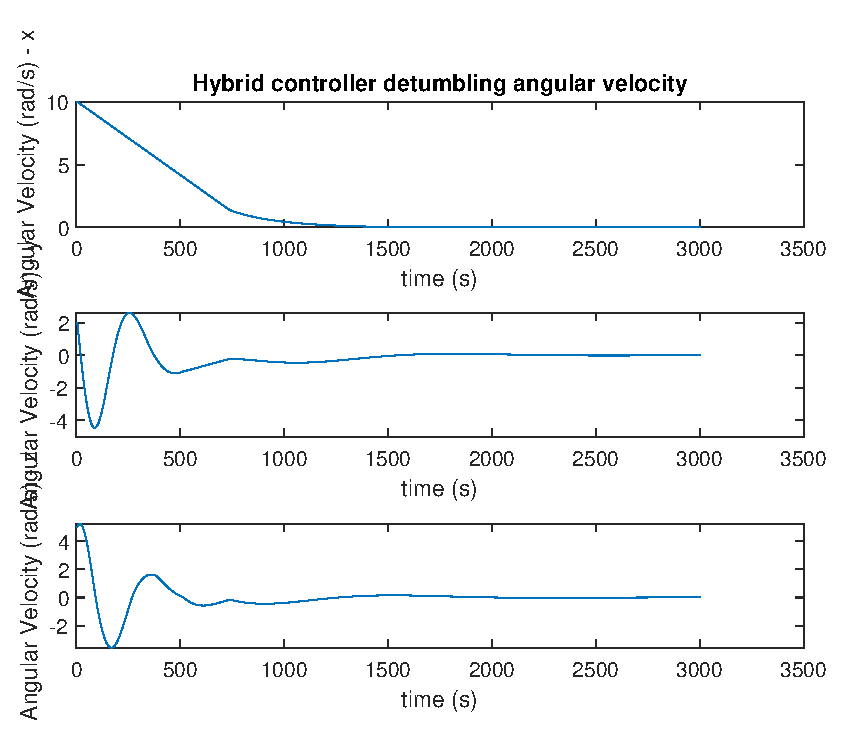
\includegraphics[width=0.7\linewidth]{figures/detumbling3}
	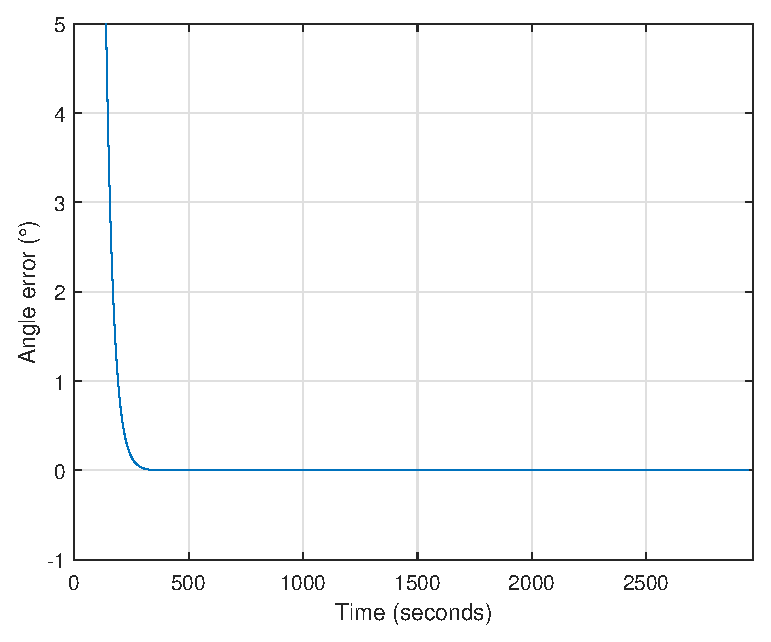
\includegraphics[width=0.7\linewidth]{figures/angle_error}
	\caption{Tracking error during nadir pointing}
	\label{fig:angle_error}
\end{figure}

Earth station tracking is  tested in a scenario where the satellite flies right over the station. This is the closest the satellite in orbit can get to the Earth station, leading to maximum torque demand. The tracking error is kept below  $1^o$, with error peaks appearing during flyover. Figures \ref{fig:angle_error2} and \ref{fig:torque_stationTrack} present the tracking error and torque demand arising during station tracking.

\begin{figure}[H]
	\centering
	%	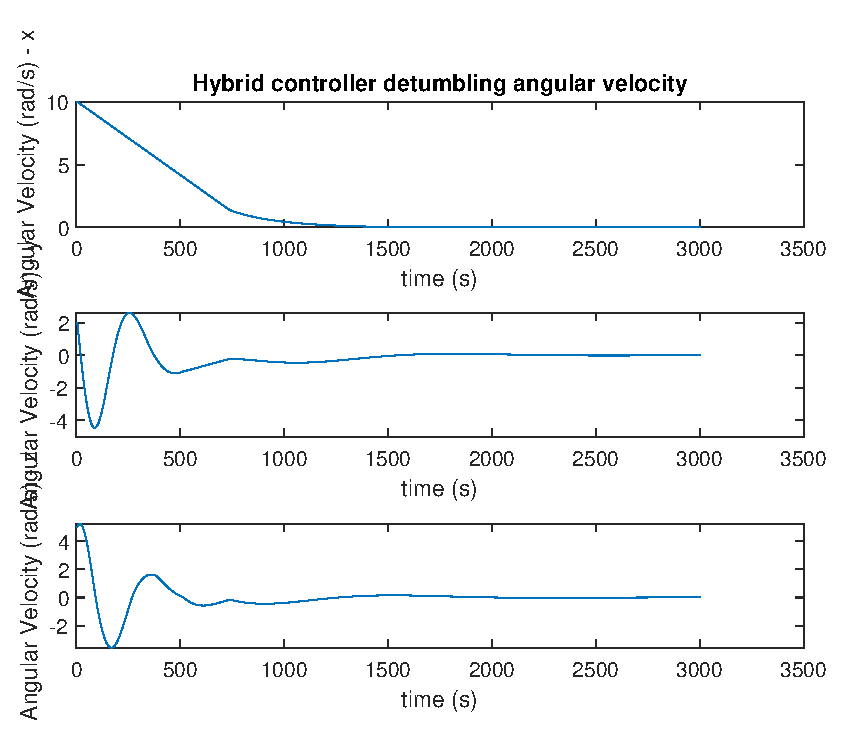
\includegraphics[width=0.7\linewidth]{figures/detumbling3}
	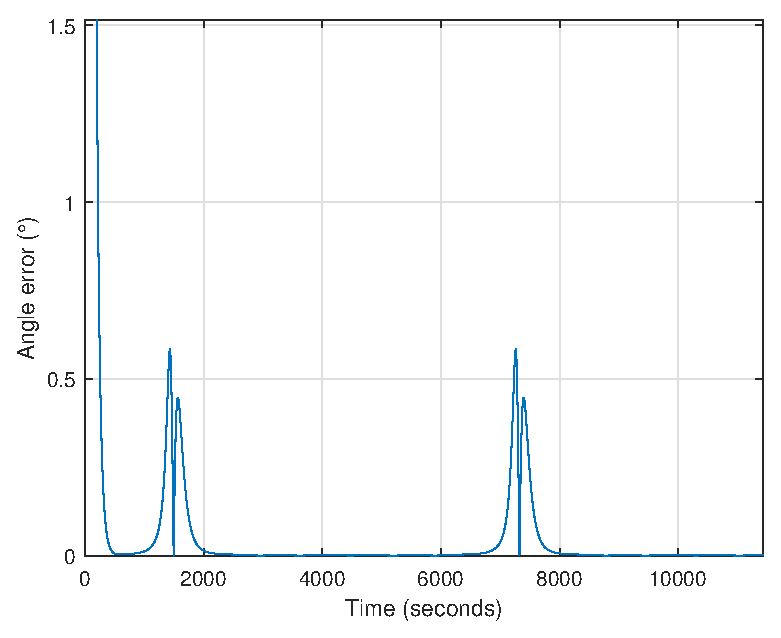
\includegraphics[width=0.7\linewidth]{figures/angle_error_stationTrack}
	\caption{Tracking error during Earth station pointing. The satellite flies over the station.}
	\label{fig:angle_error2}
\end{figure}


\begin{figure}[H]
	\centering
	%	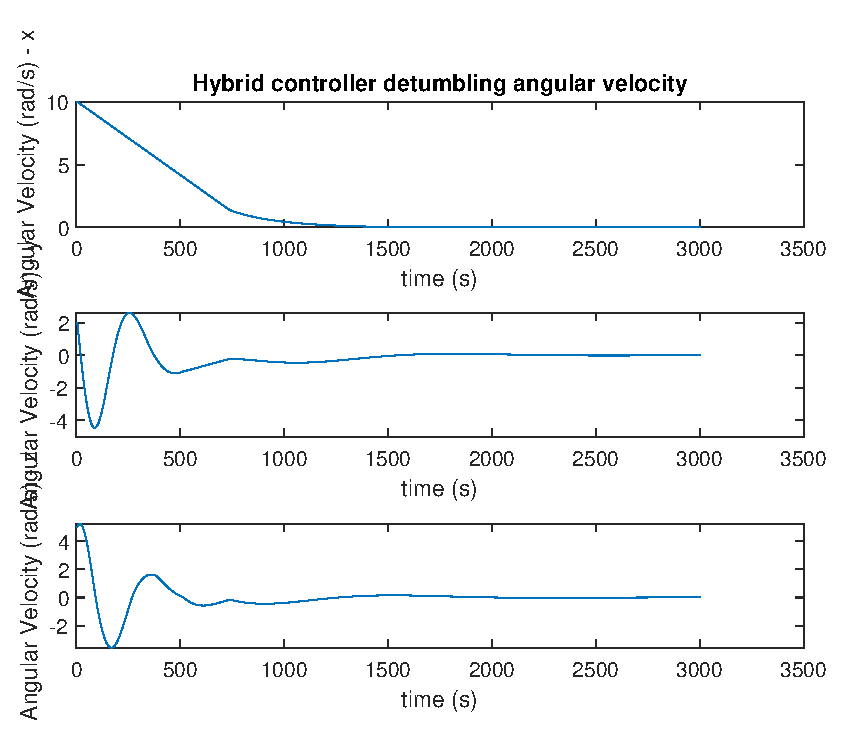
\includegraphics[width=0.7\linewidth]{figures/detumbling3}
	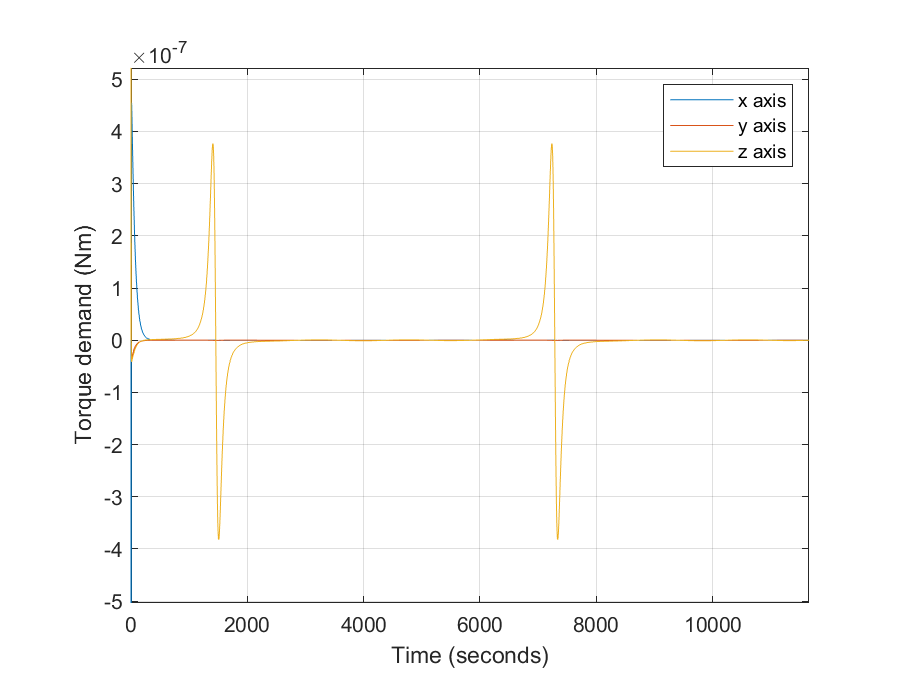
\includegraphics[width=0.7\linewidth]{figures/torque_stationTrack}
	\caption{Torque demand $\vec{u}$ during Earth station pointing. The satellite flies over the station.}
	\label{fig:torque_stationTrack}
\end{figure}

\begin{figure}[H]
	\centering
	%	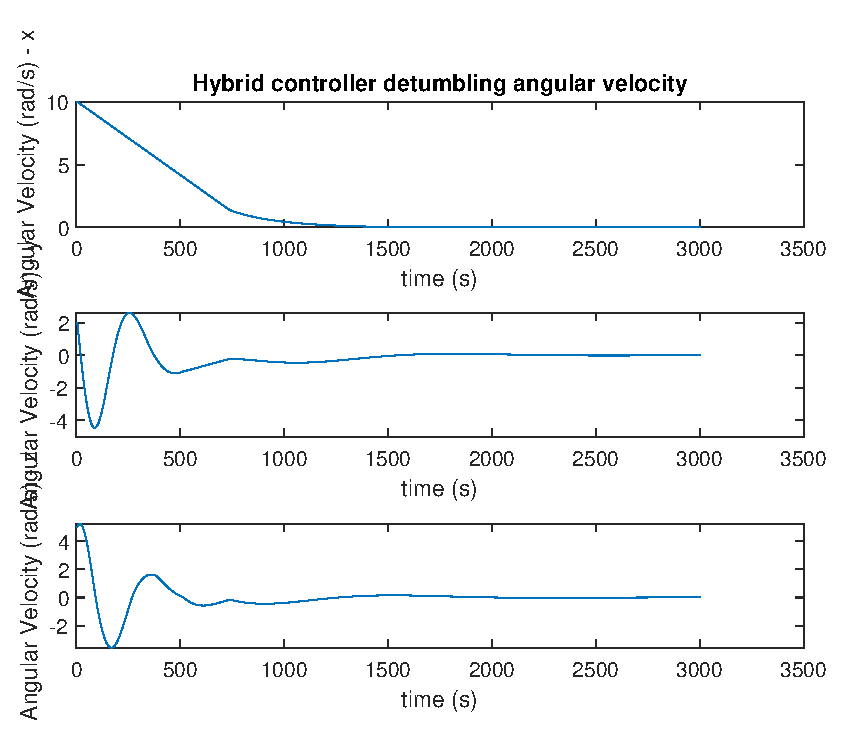
\includegraphics[width=0.7\linewidth]{figures/detumbling3}
	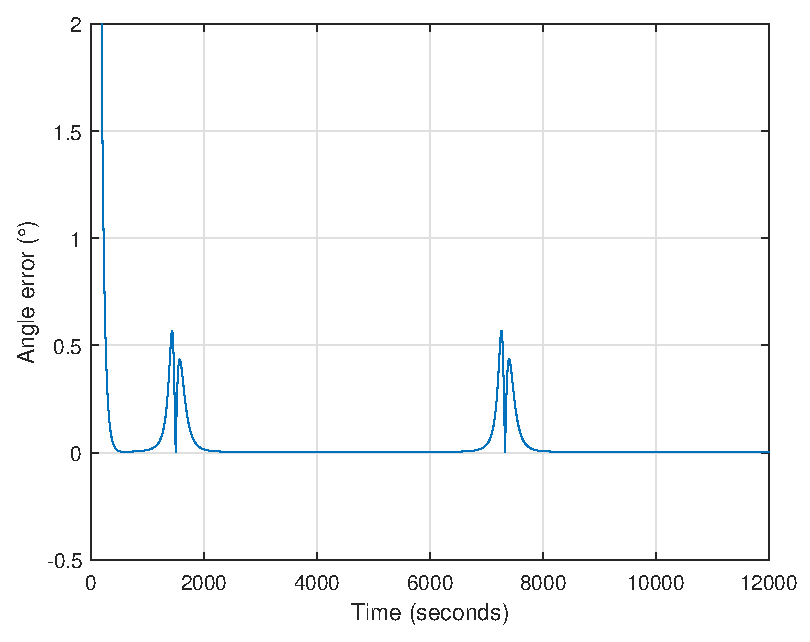
\includegraphics[width=0.7\linewidth]{figures/faultyangerror}
	\caption{Tracking error during Earth station pointing using the linear controller. The satellite flies over the station. The 3rd reaction wheel is faulty and switched off.}
	\label{fig:angle_error2}
\end{figure}


%\subsection{1. The formation shall be able to maintain a given angle within 45$^{\circ}$.}
%The

%\chapter{Conclusion}
The overall objective of this project was to consider several satellites flying in formation with the purpose of pointing towards a target. In order to reach this goal, two controllers were designed: one for controlling the angle between satellites using the drag force and another one for attitude control in order to be able to rotate the satellite to the desired orientation.

First, for designing a controller for the angle, the relative dynamics between two satellites are analyzed. Therefore, an LQR controller is implemented to control the angle between two satellites. The simulations showed that the LQR performed properly. Additionally, two algorithms for formation control are designed, a global and distributed algorithm. Both algorithms are working as intended, where the angles between neighbour satellites converged to the desired angle of 45$^{\circ}$, with the mention that in the distributed algorithm case the convergence rate will be slower compared with the global algorithm.

Afterwards, two control methods to obtain the desired orientation of the satellite has been implemented. The first method is a state feedback which is a linear control method. For implementing this controller the equation of motion need to be linearized. The second method is using a non-linear control method called sliding mode control. The results from sliding mode control showed that the error quaternion converged better compared to state feedback control, but in this case, the state feedback is deemed to be more suitable. Besides, the sliding mode convergence is better, but due to the fact that the control law is more complex, the satellite controller will need more computation time. 

In conclusion, some acceptance tests have been made to establish that the requirements accomplished. 
%
%%%% Bibliography %%%
%\printbibliography
%\cleardoublepage
%%---------- Appendix Below ----------------------------------------
%\appendix
%%\input{appendix/aTest.tex}
%\input{appendix/ServoDatasheet.tex}
%\input{appendix/Solidworks.tex}
%\input{appendix/grabberTest.tex}
%\input{appendix/colorLightTest.tex}
%\chapter{Derivation of relative dynamics equations} \label{chap:B}
The vector position from the centre of the Earth to the satellite 1 and the satellite 2 is given by
\begin{flalign}
\vec{p_1} &= R  \vec{\hat{x}} \\
\vec{p_2} &= R  \vec{\hat{x}} + x  \vec{\hat{x}} + y  \vec{\hat{y}}
\end{flalign}
the first time derivative and second time relative of $\vec{p_1}$ and $\vec{p_2}$ is computed:
\begin{flalign*}
\vec{\dot{p}_1} &= \dot{R}  \vec{\hat{x}} + R(\vec{w} \times \vec{\hat{x}}) 
\end{flalign*}
where $\vec{w}$ is the angular velocity vector and $\vec{w} = w  \vec{\hat{z}}$ due to the fact the position of the satellites stay all over the time in the plan $(\vec{\hat{x}},\vec{\hat{y}})$. Therefore, the first time derivative and the second time derivative are given by:
\begin{flalign*}
\\vec{\dot{p}_1} &= \dot{R}  \vec{\hat{x}} + w R  \vec{\hat{y}} \\
\vec{\ddot{p}_1} &= \ddot{R}  \vec{\hat{x}} + w\dot{R}  \vec{\hat{y}} + \dot{w} R  \vec{\hat{y}} + w \dot{R}  \vec{\hat{y}} + wR  (\vec{w} \times \vec{\hat{y}}) \\
&= \ddot{R}  \vec{\hat{x}} + 2w\dot{R}  \vec{\hat{y}} - w^2R  \vec{\hat{x}} \\
\vec{\dot{p}_2} &= \vec{\dot{p}_1} +  \dot{x}  \vec{\hat{x}} + x w  \vec{\hat{y}} + \dot{y}  \vec{\hat{y}} - y w  \vec{\hat{x}} \\
&= \vec{\dot{p}_1} + (\dot{x} - yw)  \vec{\hat{x}} + (xw + \dot{y})  \vec{\hat{y}} \\
\vec{\ddot{p}_2} & = \vec{\ddot{p}_1} + (\ddot{x} - \dot{y}w - y\dot{w})  \vec{\hat{x}} + (\dot{x} - yw) w  \vec{\hat{y}} + (\dot{x}w + x\dot{w} + \ddot{y})  \vec{\hat{y}} - (xw + \dot{y}) w  \vec{\hat{x}} \\
&= \vec{\ddot{p}_1} + (\ddot{x} - 2\dot{y}w - y\dot{w} - xw^2)  \vec{\hat{x}} + (\ddot{y} + 2\dot{x}w + x\dot{w} - yw^2)  \vec{\hat{y}}
\end{flalign*}
Furthermore, The Newton law gives:
\begin{flalign}
	m\vec{\ddot{p}_1} &= \vec{F_{grav,1}} + \vec{F_{drag,1}} + \vec{F_{dist,1}}	\label{eq:l3} \\
	m\vec{\ddot{p}_2} &= \vec{F_{grav,2}} + \vec{F_{drag,2}} + \vec{F_{dist,2}} 	\label{eq:l4} \\
	\Rightarrow \vec{\ddot{p}_2} - \vec{\ddot{p}_2} &= \frac{1}{m}(\Delta \vec{F_{grav}} + \Delta \vec{F_{drag}} + \Delta \vec F_{dist}) 	\label{eq:l5}
\end{flalign}
with m is the mass of both satellites. The gravity is given by the universal law of gravitation:
\begin{flalign*}
\frac{\vec{F_{grav,1}}}{m} &= -G\frac{m_{earth}}{||\vec{R}||^3} \vec{R} \\
\frac{\vec{F_{grav,2}}}{m} &= -G\frac{m_{earth}}{||\vec{R} + \vec{r}||^3} (\vec{R} + \vec{r})
\end{flalign*}
where $\vec{r} = (x,y)$ is the vector from the satellite 1 to the satellite 2. The denominateur can be approximated using:
\begin{flalign*}
||\vec{R} + \vec{r}||^{-3} &= ||\vec{r}|| \\
%||\vec{R} + \vec{r}||^{-3} &= ||(\vec{R} + \vec{r})\cdot(\vec{R} + \vec{r})||^{\frac{-3}{2}} \\
%&= ||\vec{R} \cdot \vec{R} + \vec{r} \cdot \vec{r} + 2\vec{R} \cdot \vec{r}||^{\frac{-3}{2}} \\
%&= R^{-3}||1 + \frac{\vec{r} \cdot \vec{r}}{R^2} + 2\frac{\vec{r} \cdot \vec{R}}{R^2}||^{\frac{-3}{2}}
\end{flalign*}
%Due to the fact the $r << R$, the second term can be neglected and by using the approximation $(1 + x)^q = 1 + qx$ when $x << 1$. The expression can be approximated by:
%\begin{flalign*}
%||\vec{R} + \vec{r}||^{-3} &= R^{-3}(1 - 3\frac{\vec{r} \cdot \vec{R}}{R^2}) \\
%&= R^{-3}(1 - 3\frac{x}{R})
%\end{flalign*} 
and thus, the difference between the gravity force on satellite 2 and the the gravity force on 1 is:
\begin{flalign*}
\vec{F_{grav,2}} - \vec{F_{grav,1}} &\approx -\frac{\mu}{R^3}\vec{r} \\
%\vec{F_{grav,2}} - \vec{F_{grav,1}} &\approx -G \frac{m_{earth}}{R^3} ((1 - 3\frac{x}{R}) (\vec{R} + \vec{r}) - \vec{R}) \\
%&\approx -G \frac{m_{earth}}{R^3} (\vec{r} - 3x \cdot \vec{\hat{x}} + 3 \frac{x}{R} \vec{r}) \\
%&\approx -\frac{\mu}{R^3} (-2x \cdot \vec{\hat{x}} + y \cdot \vec{\hat{y}})
\end{flalign*} 
with $\mu = G  m_{earth}$, The drag force can be modelling be using \eqref{eq:teor}:
\begin{flalign*}
	\vec{F_{drag,1}} &= -u_1 ||\vec{\dot{p}_1}|| \vec{\dot{p}_1}\\
	& = -u_1 ||\vec{\dot{p}_1}|| (\dot{R}  \vec{\hat{x}} + wR  \vec{\hat{y}}) \\
	\vec{F_{drag,2}} &= -u_2 ||\vec{\dot{p}_2}|| \vec{\dot{p}_2} \\
	& = -u_2 ||\vec{\dot{p}_2}|| ((\dot{R} + \dot{x} - yw) \vec{\hat{x}} + (wR + xw + \dot{y})  \vec{\hat{y}})
\end{flalign*}
Therefore, the \eqref{eq:l3} becomes:
\begin{equation}
\left\{
	\begin{aligned}
		&\ddot{R} - w^2R = -\frac{\mu}{R^2} -\frac{u_1}{m} ||\vec{\dot{p}_1}|| \dot{R} + \frac{F_{dist,1,x}}{m} \\
		&2w\dot{R} + \dot{w}R = -\frac{u_1}{m} ||\vec{\dot{p}_1}|| wR + \frac{F_{dist,1,y}}{m}
	\end{aligned}
\right.
\end{equation}
and the \eqref{eq:l5} gives:
\begin{equation}
\left\{
	\begin{aligned}
		& \ddot{x} - 2\dot{y}w - y\dot{w} - xw^2 = -x\frac{\mu}{R^3} + \frac{u_1}{m} ||\vec{\dot{p}_1}|| \dot{R} - \frac{u_2}{m} ||\vec{\dot{p}_2}||(\dot{R} + \dot{x} - yw) + \frac{\Delta F_{dist,x}}{m}\\
		&\ddot{y} + 2\dot{x}w + x\dot{w} - yw^2 = -y\frac{\mu}{R^3} + \frac{u_1}{m}||\vec{\dot{p}_1}||wR - \frac{u_2}{m}||\vec{\dot{p}_2}||(wR + xw + \dot{y}) + \frac{\Delta F_{dist,y}}{m}
	\end{aligned}
\right.
\label{eq:l7}
\end{equation}
The operating point is the position ($x^{*},y^{*}$) of the satellite 2 in the frame of satellite. $x^{*}$ and $y^{*}$ can be computed from \figref{fig:operating_pt}.
\begin{figure}[H]
	\centering
	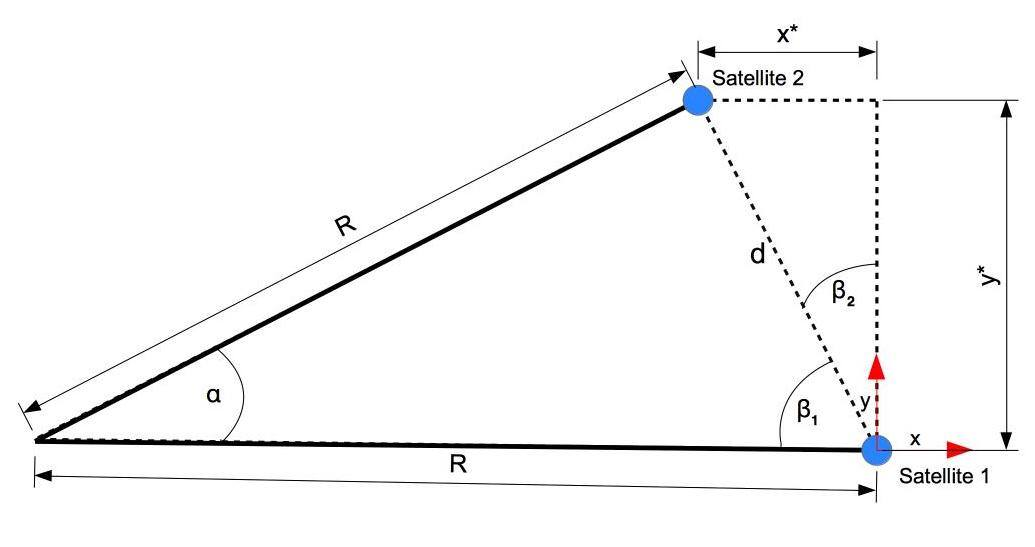
\includegraphics[width=0.75\linewidth]{figures/operating_point}
	\caption{Operating point}
	\label{fig:operating_pt}
\end{figure} 
Using trigonometry relations:
\begin{flalign*}
d &= 2Rsin(\frac{\alpha}{2}) \\
x^{*} &= -dsin(\beta_2) \\
&= -dsin(\frac{\alpha}{2}) \\
&= -2Rsin(\frac{\alpha}{2})^2 \\
y^{*}  &= dcos(\frac{\alpha}{2}) \\
&= 2Rsin(\frac{\alpha}{2})cos(\frac{\alpha}{2}) \\
&= Rsin(\alpha)
\end{flalign*}
with $\alpha$ is the desired angle between satellite and so $\beta_2 = 90^{\circ} - \beta_1 = 90^{\circ} - (90^{\circ} - \frac{\alpha}{2}) = \frac{\alpha}{2}$. Therefore we change the coordinate reference as following:
\begin{flalign*}
x &\Leftarrow x - x^{*}  \\
y &\Leftarrow y - y^{*}  
\end{flalign*}
Thus, the equations \eqref{eq:l7} become:
\begin{equation}
\left\{
\begin{aligned}
	& \ddot{x} - 2\dot{y}w - (y + y^{*})\dot{w} - (x + x^{*})w^2 = \\
	&-(x + x^{*})\frac{\mu}{R^3} + \frac{u_1}{m} ||\vec{\dot{p}_1}|| \dot{R} - \frac{u_2}{m} ||\vec{\dot{p}_2}||(\dot{R} + \dot{x} - (y + y^{*})w) + \frac{\Delta F_{dist,x}}{m}\\
	&\ddot{y} + 2\dot{x}w + (x + x^{*})\dot{w} - (y + y^{*})w^2 =\\
	& -(y + y^{*})\frac{\mu}{R^3} + \frac{u_1}{m}||\vec{\dot{p}_1}||wR - \frac{u_2}{m}||\vec{\dot{p}_2}||(wR + (x + x^{*})w + \dot{y}) + \frac{\Delta F_{dist,y}}{m}
\end{aligned}
\right.
	\label{eq:la1}
\end{equation}
%\subsection{Linearisation of the relative dynamics eqations} \label{sec:C}
%From the equations \eqref{eq:la1} and assuming that the radius is constant and the angular velocity equals to $w = \sqrt{\frac{\mu}{R^3}}$, a linearization of the system can be derived using some approximations. The state is defined as :
%\begin{flalign*}
%	s = [x \ \dot{x} \ y \ \dot{y}]^\mathsf{T}
%\end{flalign*}
%Moreover, the norm of the velocity of both satellite is assumed to be equal and to be constant ($||\vec{\dot{p_1}}|| = ||\vec{\dot{p_2}}|| = C$). Therefore, the nominal system is given by:
%\begin{equation}
%\left\{
%\begin{aligned}
%& \dot{s_1} = s_2 \\
%& \dot{s_2} = 2ws_4 - u_2\frac{y^{*}wC}{m} \\
%& \dot{s_3} = s_4 \\
%& \dot{s_4} = -2ws_2 - (u_2 - u_1)\frac{wRC}{m}
%\label{eq:statespaceassumption}  
%\end{aligned}
%\right.
%\end{equation}
%using the approximation $\dot{x}$, $y << y^{*}$ and $x, x^{*}$, $\frac{\dot{y}}{w} << R$. 
%%
%
%%%% Bibliography %%%
%%\printbibliography
%
%%%% List of Corrections
%\listoffixmes

\end{document}
